\documentclass[../thesis.tex]{subfiles}

\begin{document}



    \chapter{Analysis}
    \label{ch:analysis}


      \section{Isotherm computation}
      \label{sec:isotherm-computation}

        In the following, evaluation of the recorded raw data is presented for volumetric (\cref{subsec:volumetric-computation}) and for the optical measurements (\cref{subsec:optical-computation}).


        \subsection{Volumetric isotherm}
        \label{subsec:volumetric-computation}


          To compute the isotherms from the recorded data the experiment needs to the conducted not only with a membrane inside of the cell, but also with an empty cell. From here on, the following indices shall be used:
          \begin{align*}
              \begin{split}
                  &1 \longrightarrow \textrm{no membrane} \\
                  &2 \longrightarrow \textrm{membrane}.
                  \label{eq:index_assignments}
              \end{split}
          \end{align*}
          Furthermore, the variables $P_i$, $\dot{P}_i$, $V_i$, $T_i$, $n_i$ and $\dot{n}_i$, $i\in \{1,2\}$, refer to the values measured inside of the cell, in explanation the red marked part of the system in \cref{fig:setup-bypass}. The raw isotherms of the two experiments are shown in \cref{fig:raw-isotherms}. The plateaus of the yellow curve with membrane inside the cell of the plot versus time  correspond to the dips of the time derivative of the pressure of the versus pressure plot. This can be explained by the hexane condensing inside the membrane's pores at a given pressure due to which the continuing matter flow into the cell does not yield an increase of pressure.
          \medskip

          \subfile{tikz/graphs/295b_membrane_vs_nomembrane/295b_membrane_vs_nomembrane.tex}

          Regarding the system with and empty cell, it is clear that the ideal gas law can be used to compute the flow rate of hexane (compare \cref{sec:ideal-gas-law}). By solving for the amount of matter
          \begin{equation*}
              n_1 = \frac{P_1V_1}{RT_1},
          \end{equation*}
          taking into account that the temperature of the cell is regulated at $T_1$ and the volume $V_1$ is constant, the flow of matter becomes
          \begin{equation*}
              \dot{n}_1 = \frac{V_1}{RT_1}\cdot \dot{P}_1.
              \label{eq:n1}
          \end{equation*}
          Furthermore, the flow of matter for the system with a membrane inside the cell can be interpreted as the sum of the flow into the membrane $\dot{n}_2^\mathrm{mem}$ and the flow into the system volume excluding the membrane $\dot{n}_2^\mathrm{cell}$. This can be rewritten yielding
          \begin{equation*}
              \dot{n}_2^\mathrm{mem} = \dot{n}_2 - \dot{n}_2^\mathrm{cell},
          \end{equation*}
          where $\dot{n}^\mathrm{cell}_2$ obeys ideal gas law. Using the fact that the flow through the \textsc{Pfeiffer} valve only depends on the pressure difference $\Delta P_i = P_i^\mathrm{tank} - P_i^\mathrm{cell}$, assuming that $P_1^\mathrm{tank} = P_2^\mathrm{tank}$ leads to
          \begin{align}
              \begin{split}
                  \dot{n}_2^\mathrm{mem}(P_2) &= \dot{n}_1(P_2) - \dot{n}_2^\mathrm{cell}(P_2)\\
                  &=\frac{V_1}{RT_1}\cdot \dot{P}_1(P_2) - \frac{V_2}{RT_2}\cdot \dot{P}_2(P_2)
              \end{split}
              \label{eq:ndot-membrane}
          \end{align}
          \Cref{fig:iso-computation} shows the computation steps visually using the respective plots versus time.

          \subfile{tikz/graphs/295d_integration_visualization/295d_integration_visualization.tex}

          As the temperature of the system is regulated ($T = T_1 = T_2 = \mathrm{const.}$) and because $V = V_1 \approx V_2$ since $V_\mathrm{mem} \ll V_1$, equation \cref{eq:ndot-membrane} yields
          \begin{equation}
              n_2^\mathrm{membrane} = \frac{V}{RT}\int_0^{t_2}\left(\dot{P}_1(t_1') - \dot{P}_2(t_2')\right) \mathrm{d}t_2'.
              \label{eq:nmembrane-1}
          \end{equation}
          Important at this point is the dependency of $\dot{P}_1(t_1)$ on $t_1)$ while the integration is over $t_2$.

          As the experimental setup yields discreet values at given time intervals $\Delta t$, the data evaluation makes use of a sum rather than an integration.
          \begin{equation}
              n = \frac{V}{RT} \sum \left( \dot{P}_1 ( P_1 = P_2) - \dot{P}_2(P_2) \right) \cdot \Delta t
              \label{eq:nmembrane}
          \end{equation}
          yields the molar amount of hexane condensed inside the membrane. Figure \cref{fig:iso} shows the result of the integration \cref{eq:nmembrane} for membrane 296d. It is a absorption and desorption isotherm for hexane inside the porous alumina membrane. The bulk condensation and evaporation is not visible, as it is also recorded with the reference isotherm without membrane inside the cell.

          What stings the eye is that the sharp rise of the condensation branch does not start at the liquid fraction $LF=0$. The same goes for the evaporation branch. It only drops to a liquid fraction value $LF>0$ and then decreases superimposed with the condensation branch. While is would be reasonable to renormalize the graph so only the mentioned sharp rise and drop are relevant for the isotherm as this part is where the pores fill or empty at spinodal or equilibrium pressure (\cref{sec:cond_evap_theory}), it is not done here. The reason for this is that the initial rise of the isotherms is assumed to be due to the build up of a film on the membranes surfaces. This is part of the theory of condensation and evaporation in confinement even though the film is ignored in the basic \textsc{Kelvin} equation (\cref{sec:kelvin-equation}). ???MAKE A COMPUTATION AS TO HOW MANY MOLES OF LIQUID ARE EXPECTED FOR THE FILMS ON ONE SINGLE MEMBRANE???
          \medskip

          Moreover, the plots
          \begin{equation}
              i \quad \mathrm{over} \quad j,\quad i\in \{n,LF,FF\}, \quad j\in \{P_\mathrm{cell},P_\mathrm{rel},D_\mathrm{kelvin}\}
          \end{equation}
          are of interest, where
          \begin{equation}
              P_\mathrm{rel} = \frac{P_\mathrm{cell}}{P_\mathrm{sv}^\mathrm{exp}},
          \end{equation}
          with the saturated vapor pressure $P_\mathrm{sv}$.
          \begin{equation}
              LF = \frac{n}{n_\mathrm{max}}
          \end{equation}
          is the liquid fraction of hexane condensed inside the pores of the membrane using the total maximum amount of condensed hexane $n_\mathrm{max}$ and last,
          \begin{equation}
              FF = \frac{V_\mathrm{hex}^\mathrm{cond}}{V_\mathrm{mem}}
          \end{equation}
          with the volume of condensed hexane $V_\mathrm{hex}^\mathrm{cond}$ and the membrane's volume $V_\mathrm{mem}$, is the filled fraction of the membrane. Its maximum corresponds to the porosity of the membrane. For the computation please refer to \cref{subsec:porosity}.

          For the computation of the introduced physical sizes, the saturated vapor pressure $P_\mathrm{sv}$ must be determined.


          \subsubsection{Porosity}
          \label{sssec:porosity}

            Equation \cref{eq:nmembrane} gives the molar amount of hexane $n_\mathrm{hex}$ condensed inside the membrane's pores. Furthermore, for the given pressures $\SIrange{0}{160}{\milli\bar}$ hexane in its liquid form can be regarded as incompressible and therefore the hexane's volume be computed via
            \begin{equation*}
                V_\mathrm{hex} = n_\mathrm{hex} \cdot V_\mathrm{mol, hex}.
            \end{equation*}.
            The thickness $l_\mathrm{pore}$ of the membrane is easily determinable via MEB views since its magnitude is micrometers. Finally, the area $A_\mathrm{mem}$ of the measured samples is derived from a photo taken using binoculars.

            Using these information the porosity $\phi$ of a given membrane is given by
            \begin{equation}
                \phi = 1 - \frac{V_\mathrm{hex}}{V_\mathrm{mem}} ,
                \label{eq:porosity}
            \end{equation}
            with the membrane's volume
            \begin{equation*}
                V_\mathrm{mem} = A_\mathrm{mem} \cdot l_\mathrm{pore}.
            \end{equation*}


          \subsubsection{Determination of the saturated vapor pressure}
          \label{sssec:determination-sat-vapor-pressure}

            As the bulk condensation plateau shows a slight drift (compare figure \cref{fig:raw-isotherms}), using the maximum measured pressure $P_\mathrm{cell}$ does not yield the saturated vapor pressure $P_\mathrm{sv}$ but a higher value. In addition, depending on the contamination of the system by air or degassing grease, the measured value for $P_\mathrm{sv}$ shifts due to the partial pressures. To probe the reproducibility of an isotherm loop including the grade of contamination, the  node[anchor=south]maximum measured pressure for different membranes is compared. As the system is opened to replace the membrane in between the isotherms, each cycle is independent. For the change of membrane process please read \cref{sssec:changing-the-sample}. The result of the experiment is that $P_\mathrm{sv}^\mathrm{exp}$ fluctuates by
            \begin{equation}
                \delta P_\mathrm{sv}^\mathrm{exp} = \pm \SI{0,5}{\milli\bar}.
                \label{eq:delta-Psat}
            \end{equation}
            As the relevant plateau of condensation and evaporation inside the pores of the membrane occur at about
            \begin{equation}
                P_\mathrm{plateaus} = \SI{140}{\milli\bar},
            \end{equation}
            $\delta P_\mathrm{sv}^\mathrm{exp}$ translates to an error of about
            \begin{equation}
                \delta P_\mathrm{rel} \le \pm 0,005.
                \label{eq:delta-Prel}
            \end{equation}


          \subsubsection{Diameter error using Kelvin equation}

            \textsc{Gaussian} error propagation to check the precision of the experiment.


        \subsection{Optical measurements}
        \label{subsec:optical-computation}

          As mentioned in \cref{sec:exp-setup}, the light transmission setup is independent from the volumetric measurements and also the evaluations do not depend on each other. The light transmission is rather a tool to check on the theory of evaporation and condensation within the membrane using a different approach.
          \medskip

          To compute the transmission coefficient of a membrane, it is measured in dry state using the same transmission setup as during the volumetric experiment yielding $T_\mathrm{mem}^\mathrm{dry}$. Then, the first measured intensity value $I_0$ of a given isotherm is assigned to the dry coefficient as at this point no hexane is condensed inside of the membranes pores yet. From there on, each intensity measurement is translated to a transmission coefficient according to
          \begin{equation}
              T(t) = T_\mathrm{mem}^\mathrm{dry} \cdot \frac{I_0}{I(t)}.
          \end{equation}
          The aquired physical size can be interpreted as explained in the following  \cref{subsec:light-transmission-interpretation}.

          As a forword shall be mentioned that the observed transmission drops' magnitude cannot be explained by simple media transmissions as explained in \cref{subsec:two_interface_trans}. Even counting multiple transitions for a diagonal transmission of a membrane, the regular transmission is not a sufficient explanation as the filled state of a membrane should by that theory be less transmitting than the empty state whereas the opposite is observed. To explain the phenomena, \textsc{Rayleigh} scattering and index matching, which are explained in \cref{sec:rayleigh-scattering} and \cref{sec:index-matching} respectively, must be taken into account.


      \section{Conducted measurements}
      \label{sec:conducted-measurements}

        \subfile{tikz/wafers/wafer_processing_plans.tex}

        Genereal: From one wafer we can test different things as we have 12 membranes. Wafer produced as a whole so membranes should be equivalent. ADD THE CIRCLE HERE!!!
        \medskip

        Membranes of four different wafers produced according to \cref{subsec:membrane-production} have been measured. The wafers specifications are noted in \cref{tbl:wafer-specifications}. As multiple membranes in the same state of the same wafer yielded different results, the position of the single membranes on the wafer were are taken note for newly produced wafers. Therefore, for the wafers 295 and 296, the membranes' names correspond to the positions shown in \cref{fig:membrane-distribution}. Furthermore, all conducted measurements on the membranes in different states are noted on \cref{fig:wafer-processing-plans}.

        \subfile{tikz/wafers/membrane_distribution.tex}

        \begin{table}[htb]
          \caption{Wafer specifications. The wafers thickness $l_\mathrm{pore}$, floating time $t_\mathrm{float}$ of the \textit{barrier layer} dissolution process and pore diameter dispersion $\Delta d_\mathrm{pore}^\mathrm{MEB}$ measured by electron beam microscopy are noted. The latter two parameters apply to the open pore membranes of the respective wafer.}
          \label{tbl:wafer-specifications}
          \selectfontsize{10pt}
          \begin{tabu} {X[r]X[r]X[r]X[r]}
            \unitoprule \\
            \textbf{Wafer} & \textbf{$l_\mathrm{pore}$ $[\si{\micro\meter}]$} & \textbf{$t_\mathrm{float}$ $[\si{\minute}]$} & \textbf{$\Delta d_\mathrm{pore}^\mathrm{MEB}$ $[\si{\nano\meter}]$} \\
            \unimidrule \\
            292 &60  &0   & \\
            294 &60  &0   &  \\
            295 &60  &35  &  \\
            296 &30  &40  &7   \\
            \unitoprule \\
          \end{tabu}
        \end{table}


      \section{Inhomogeneities on one wafer}
      \label{sec:wafer-inhomogeneities}

        To start with, the wafers shall be tested for inhomogeneities. Therefore, isotherms of one wafer's membranes which are in the same technical state, meaning they have undergone exactly the same treatments, asrae compared. This is done for both, closed pore membranes and open pore membranes. Because opening the membranes' pores involves one more production step, here, closed pore membranes are regarded first.

        \Cref{fig:inhomogeneities-cp} shows a comparison of closed pore membranes for wafer 295 and 296. Even though the membranes 296e' and 296f' had already been treated using phosphoric acid at the time of the measurements, the pores are still assumed to be closed as will be explained in \cref{sec:comparison-cp-op}.

        While for both wafers, with one exception being membrane 295c, the overall shape of the different membranes' volumetric isotherms matches, they are distributed along a short distance of the $P_\mathrm{rel}$-axis. As long as the shapes and also the size of the hysteresis match, this can be explained by a differing pore size distribution for the different membranes. NEED DIAMETER CONVERSION FOR THIS??? Membrane 295c shall not be analysed at this point as it will be dealt with in detail in \cref{sec:theory-and-defects}. Moreover, also the transmission measuremens yield optical signals of similar shapes. Unclear at this point is the variation in magnitude that can be extreme for some membranes as the example of 296f' compared to 296b shows.

        \subfile{tikz/graphs/wafer_inhomogeneities/inhomogeneities_cp.tex}

        \subfile{tikz/graphs/wafer_inhomogeneities/inhomogeneities_op.tex}


      \section{Comparison of closed and open pores}
      \label{sec:comparison-cp-op}

        Show comparison of 294, 295 and 296. Speak about the context to theory. Testing the efficiency of opening procedure. Theory test relies on the fact that pores are well open. ADD ONE THAT DID NOT WORK

        Hysteresis for closed: corrugations

        Hysteresis difference: Coherent with theory
        \medskip

        This section shall serve to determine a systematic change of the isotherm by the \textit{barrier layer} dissolution process which opens the pores on the bottom side. Moreover, the coherence with theory shall be regarded. \Cref{fig:op-cp-comp} shows the comparisons of closed pore and open pore membranes of the wafers 295 and 296. For both, closed and open pore measurements, the same membranes are used before and after the \textit{barrier layer} dissolution to leave no doubt as to the inhomogeneities of the wafers.

        \subfile{tikz/graphs/cp_op_comp/cp_op_comp.tex}

        Firstly, in reference to the model explained in \cref{sec:cond_evap_theory}, the occurence of a hysteresis for the volumetric isotherm of a closed pore membrane must be explained. The answer to that question has already been given by (???cite bruschi???): It occurs due to intra pore corrugations. The modulation of the diameter along the pore's length corresponds to a varying equilibrium pressure. This makes for a non vertical isotherm.

        Next,the difference between the isotherms for closed and open pores is regarded. Clearly, the size of the hysteresis increases. This tendency is coherent with theory as the latter predicts a hysteresis for open pores but as mentioned above, none for closed pores. Moreover, the evaporation branch of the open pore isotherm is shifted towards higher pressures as compared to the closed pore isotherm. That implies an increase of the pore diameter upon dissolving the \textit{barrier layer}.
        \medskip

        To prove that all the closed pore membranes of wafer 296, of which some have been treated using phosphoric acid, are indeed closed pore membranes, they are added to the graph of the membranes 296b and 296b' as shown in \cref{fig:full-comp-w296}. The comparison of the different membranes yields a significant difference of the hysteresis' size of 296b op and all other membranes, which show a much smaller hysteresis. As the size of the hysteresis for the rest of the membranes is approcimately uniform and the variation of the condensation and evaporation pressures are only slighty shifted, this implies that indeed, all membranes except 296b op contain pores open only on one end. Which cannot be observed though, that is weather the pores already have microscopic openings on the barrier layer side. If that were the case, hexane would condense there at spinodal pressures lower than the equilibrium pressure of the small ends. Hereby, the pores would be left in a closed shape. This case would not be visible on the volumetric measurements as the condensed amount of hexane necessary to close the pores were so small. If the openings were so large already as for the spinodal pressure to be larger than the equilibrium pressure of the small end, in explanation
        \begin{equation}
          P_\mathrm{sp}(d_\mathrm{pore})\le P_\mathrm{eq}(d_\mathrm{pore}),
        \end{equation}
        where $d_\mathrm{pore}$ is the small end's pore diameter, that case would be visible on the isotherm because whole pores would fill at higher pressures. Therefore, the latter case can be excluded.

        \subfile{tikz/graphs/296_membranes/296_membranes.tex}


        \subsection{Bad open pores}

          Talks about 294 and leads to


        \subsection{Inverse funnelling}
        \label{subsec:inverse-funnelling}

          What stings the eye of the attentive reader is that the evaporation branch also becomes more sharp for the open pores.

          An explanation of the latter two phenomena can be taken from the production step of the \textit{barrier layer} dissolution. As displayed in \cref{fig:milky-aspects}, the wafer at some point becomes milky. Comparing these milky aspects to images taken during the condensation process of an isotherm as displayed in ??? leads to the conclusion, that at this point some of the pores start filling or are already filled with phosphoric acid. This phenomena lasting for a couple of minutes is followed by fifteen more minutes of floating until the wafer is completely covered by acid that flowed through the now open pores (compare \cref{fig:filmed-membrane}). That means during at least
          \begin{equation}
            t_\mathrm{filled}=\SI{15}{\minute}
          \end{equation}
          the pores are filled by phosphoric acid. That at the end of the process, the wafer is covered by a clearly visible layer of acid, means that there must be some flux of acid through the pores. On the other hand, taking into account the sharpening evaporation branch of the volumetric isotherms implies either a sharpening pore size distribution or a decrease of the funnellization or corrugation aspect of the pores.

          By linking the occuring milky aspects to the filling of only some of the pores, meaning not all pores fill at the same time but over a span of
          \begin{equation}
            t_\mathrm{milky}=\SI{3}{\minute},
          \end{equation}
          implies that the pore size distribution should rather be increased than decreased. Excluding this point only leaves corrugations and funnellization as explanations for the sharpening isotherms. As there is no reason to believe that an etching process could flatten a corrugated surface though, the straightening of the pores is more likely. Moreover, this inverse funnelling could be explained by the acid saturating along the axis of the pores. The theory of inverse funnelling is probed by experiments that will be analysed in \cref{subsec:inverse-funnelling}.

          \begin{figure}[htpb]
            \centering
            \subfloat[]{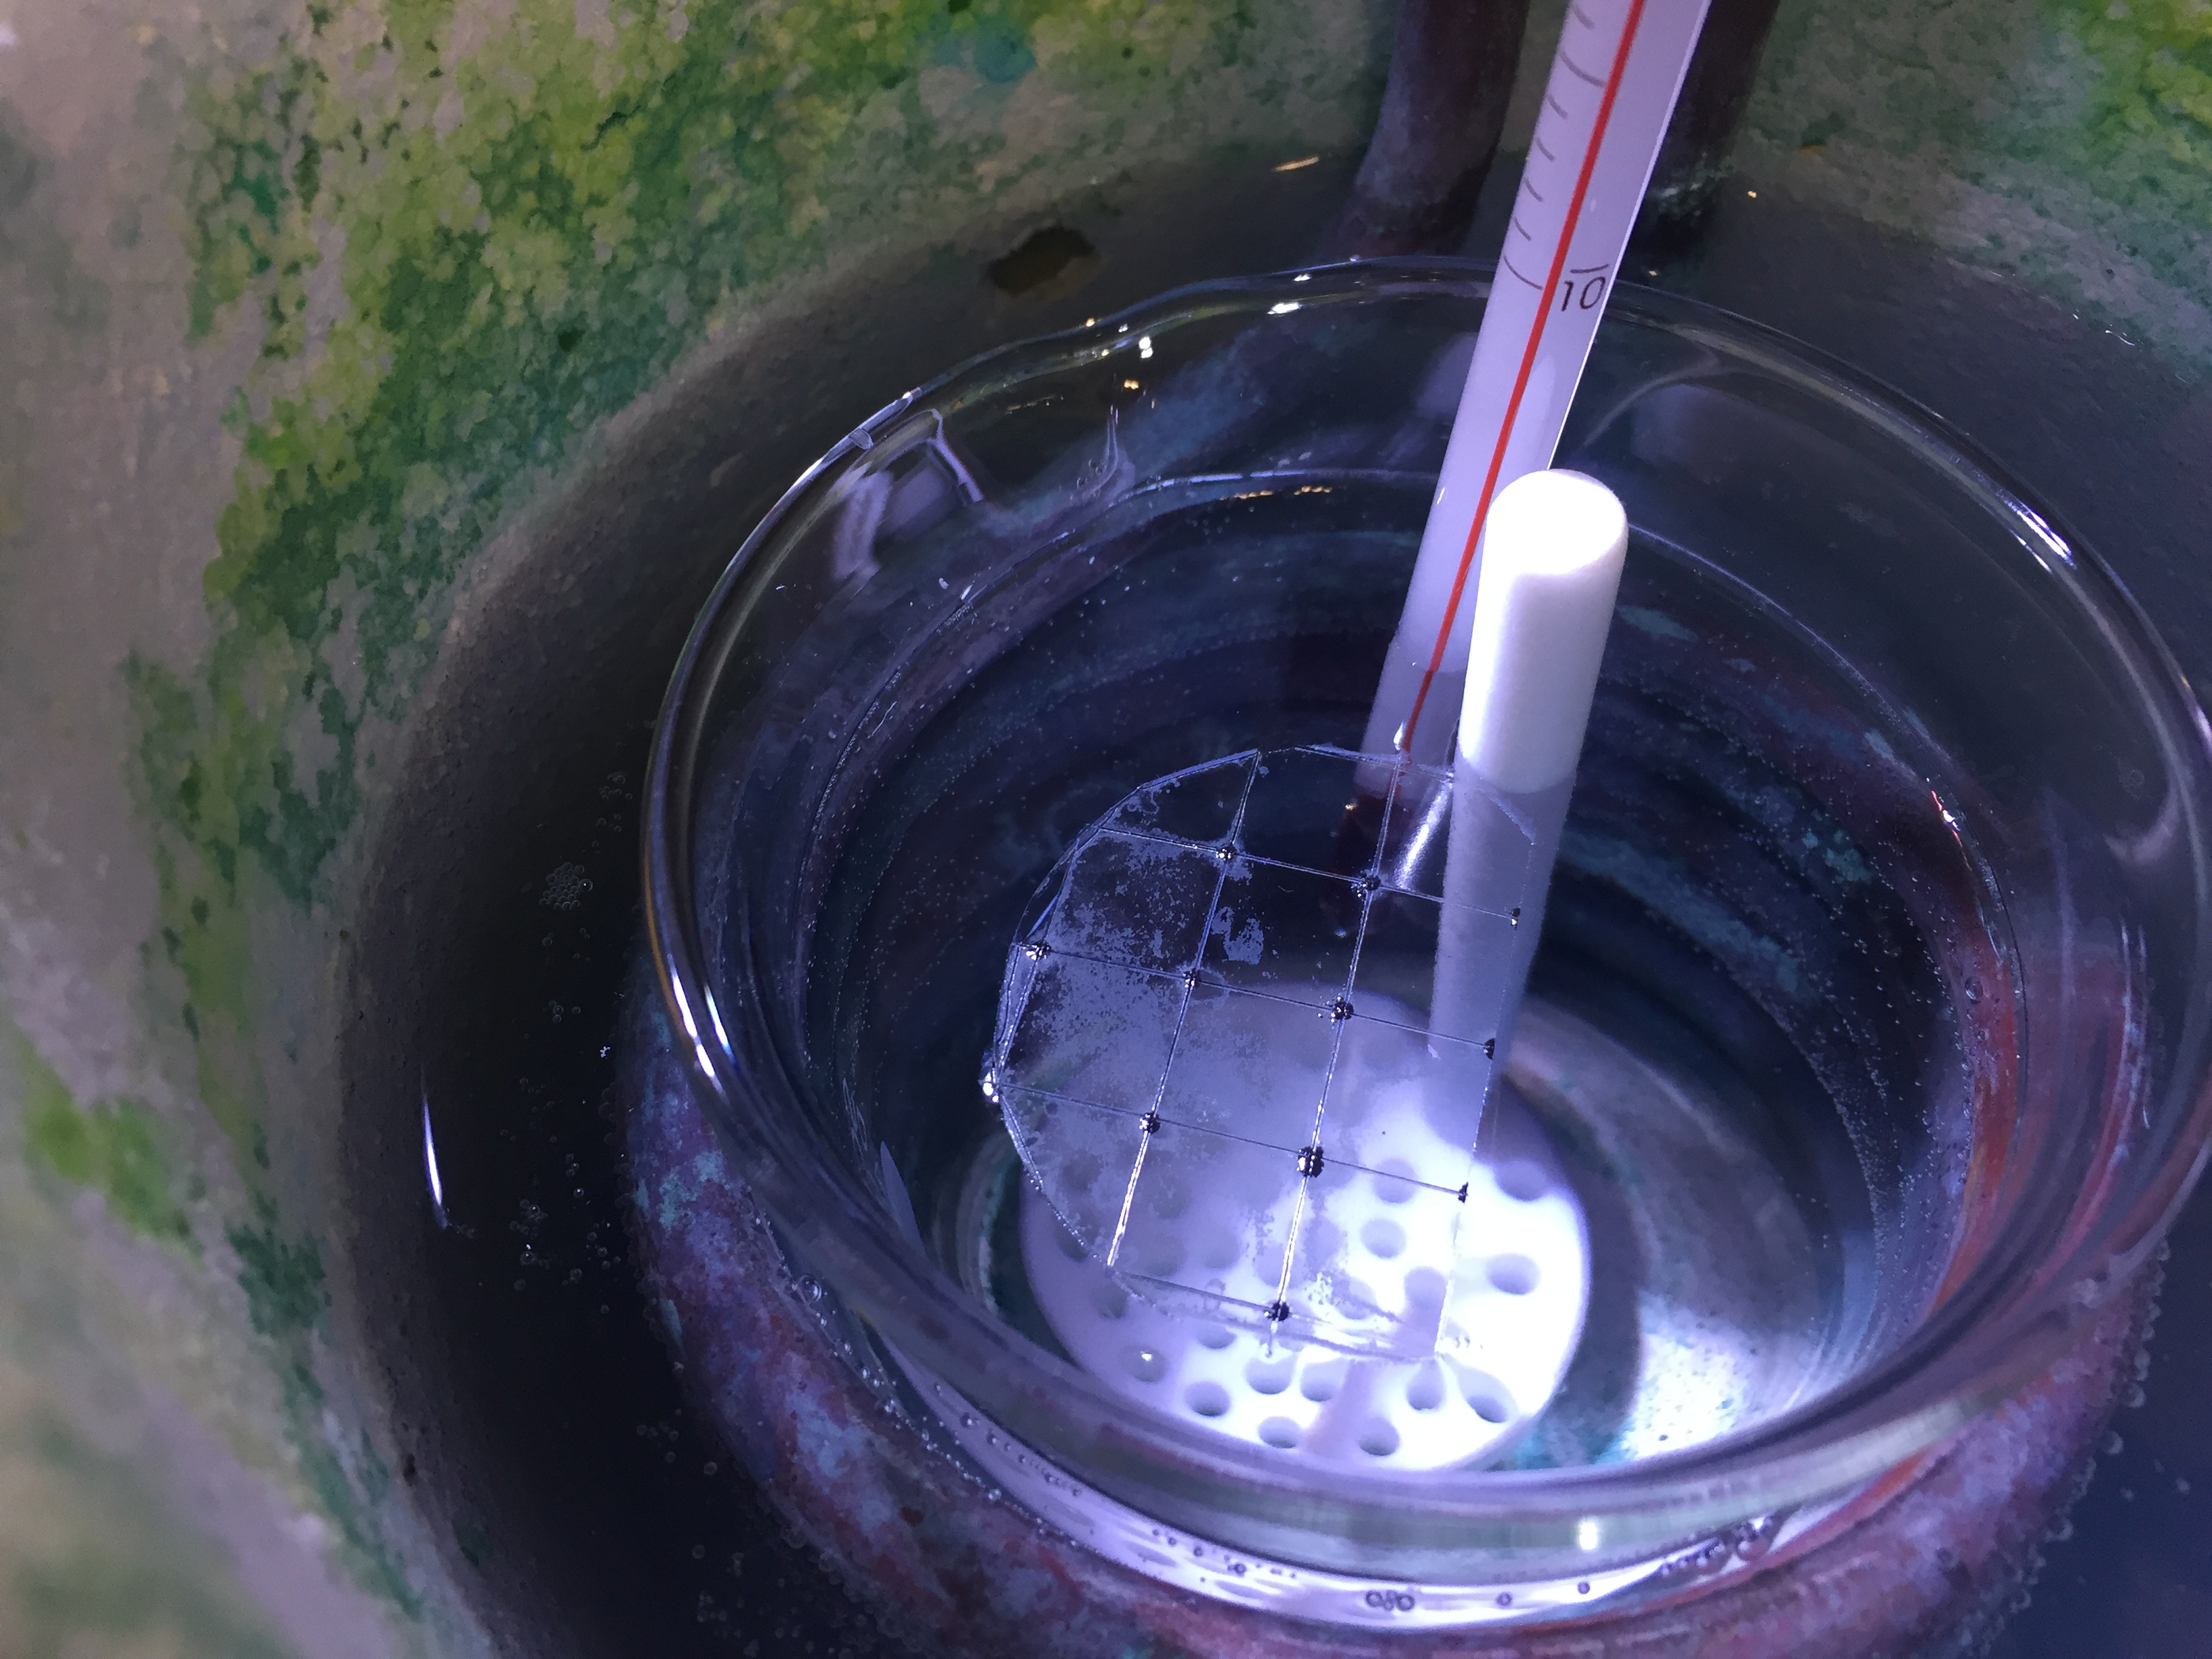
\includegraphics[width=0.45\textwidth]{images/milky_aspects.JPG}
            \label{fig:milky-aspects}}
            \hfill
            \subfloat[]{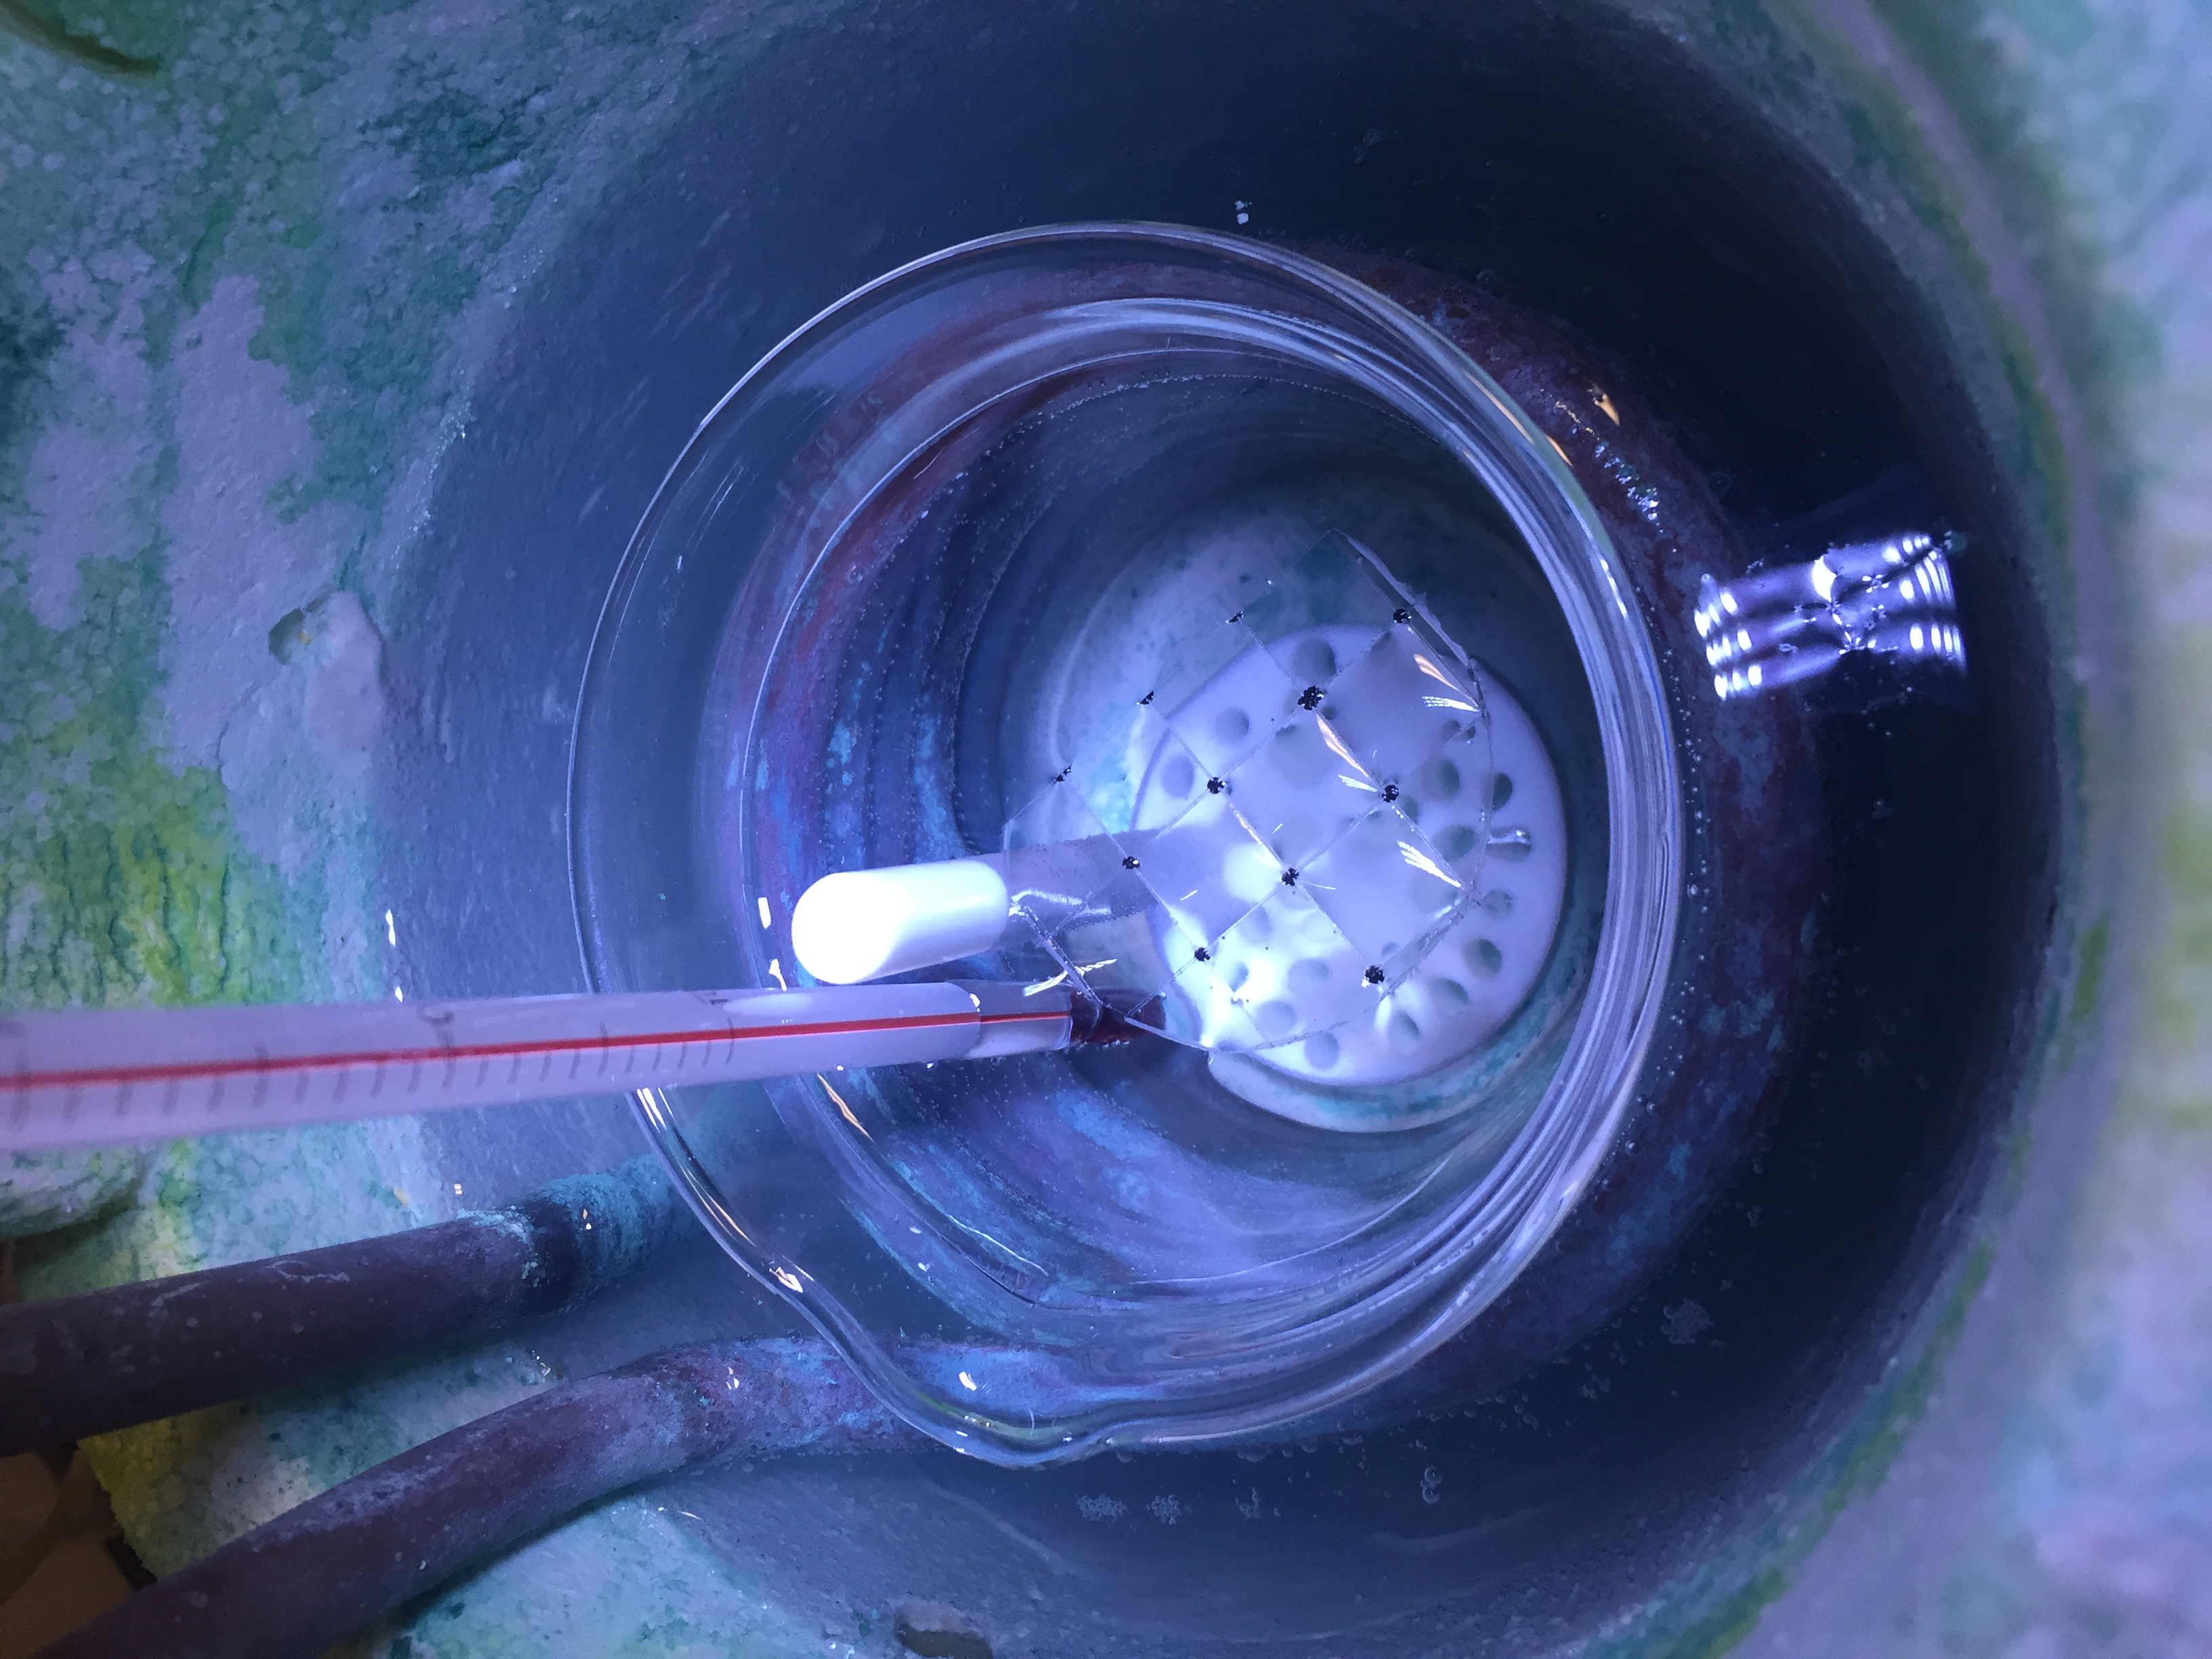
\includegraphics[width=0.45\textwidth]{images/filmed_membrane.JPG}
            \label{fig:filmed-membrane}}
            \caption{Images taken of wafer 295 during the \textit{barrier layer} dissolution process. \protect\subref{fig:milky-aspects} shows milky aspects that appear after approximately twenty minutes while \protect\subref{fig:filmed-membrane} has been taken just before removing the wafer from the acid. At this point the whole surface of the wafer is covered by phosphoric acid that passed through the pores.}
            \label{fig:barrier-layer-diss-images}
          \end{figure}


            \subsubsection{Immersion experiment}
            \label{subsec:immersion-experiment}

              Derive and explain etch rate gradient and influence on the pores' shape.
              \medskip

              Understanding the inverse funnelling becomes one of the main goals of the experimens with wafer 296 as it might be used to correct the shapes of the pores of a given membrane. Therefore, immersion experiments where two closed pore membranes are immersed in phosphoric acid for
              \begin{equation}
                \begin{split}
                  t^\mathrm{296c'}_\mathrm{im}=\SI{6,5}{\minute},    \\
                  t^\mathrm{296d'}_\mathrm{im}=\SI{13}{\minute},
                \end{split}
                \label{eq:immersion-times}
              \end{equation}
              and then the shapes of the volumetric isotherms compared to each other and addition with an untreated closed pore membrane. Focus lies on the shape of the isotherms. Small shifts in diameters are of no interest as the inhomogeneity of the pore size distributions of a wafer has been proven already in \cref{sec:wafer-inhomogeneities}.

              \subfile{tikz/graphs/immersion_experiment/immersion.tex}

              \Cref{fig:immersed-comp-w296} compares the volumetric and also the transmission measurements of the immersed membranes 296c and 296d, again adding the untreated membrane 296a. As explained in \cref{sssec:cfp-leo}, condensation and evaporation in a closed funnelled pore occur at equilibrium pressure. Pores that are open on the large end start filling from the bottom and evaporating from the top so, regarding the isotherms in \cref{fig:immersed-comp-w296}, the lower end of the isotherm rising represents the small bottom end of the pores. This lower end of all three isotherms seems to be superimposed while the top end, representing the large open end of the pores, moves to larger diameters for longer immersion times. As the effect seems to occur linearly over the whole length of the pores, the acid seems to be saturating within the pores losing etching power. By \cref{sssec:cfp-leo}, the process can be visually interpreted as a pore straightening as shown in \cref{fig:funneling_increase}. Moreover, the increase of the funnelling aspect seems to be linear at least within the first 13 minutes of the immersion as doubling the immersion time yields double the diameter shift on the volumetric isotherm (compare \cref{eq:t-immerse}). For instance, \cref{tbl:etch_rate} shows the diameter increase of the pores due to the immersion of the membranes in phosphoric acid. Using this data along with the assumption of a linear etch rate gradient along the length of the pore, the respective etch rate can be plotted as shown in \cref{fig:etch_rate_plot}. Here, the parameter $h$ is used as the height within a vertical pore, where $h=\SI{60}{\micro\meter}$ refers to the open top end of a $\SI{60}{\micro\meter}$ long pore that is closed on the bottom side. The effect, that reduces the funnelling aspect of the pores when floating the membranes on phosphoric acid as to dissolve the \textit{barrier layer} shall be referred to as \textit{inverse funnelling} from now on.

              \begin{table}
                \caption{Diameter reduction per minute of immersion derived from the isotherms of the membranes 296a, 296c, 296d.}
                \label{tbl:etch_rate}
                \selectfontsize{10pt}
                \begin{tabu} {X[r]X[r]X[r]}
                  \unitoprule \\
                  \textbf{$t_\mathrm{im} [\si{\minute}]$} & \textbf{$\Delta d_{h=\SI{60}{\micro\meter}} [\si{\nano\meter}]$} & \textbf{$\Delta d_{h=\SI{0}{\micro\meter}} [\si{\nano\meter}]$} \\
                  \unimidrule \\
                  0 &0  &0 \\
                  6,5 &3  &0  \\
                  13  &6  &0  \\
                  \unitoprule \\
                \end{tabu}
              \end{table}

              As for the transmission measurements, the shifts of the beginning of the condensation dip and also the end of the evaporation dips correspond to the interpretation explained above. Ob the other hand, the magnitude difference of the three isotherms' dips cannot be explained, neither interpreted at this point.

              \subfile{tikz/wafer_analysis/funnelling_increase.tex}


            \subsubsection{Inverse funnelling upon barrier layer dissolution}
            \label{subsec:pore-opening-effect}

              Explain that the pores appear to be straightened bc of floating. Refer to the theory, that there are two sorts of alumina (pure and acid  polluted).
              \medskip

              With the conclusions reached in \cref{subsec:immersion-experiment}, it is clear now that indeed, the \textit{barrier layer} dissolution process reduces the funnellization of the pores. One more thing still does not fit into the great picture, though, which is that the kink of the volumetric isotherm of membrane 295b (compare \cref{fig:295b_op_cp_comp}) disappears uppon pore opening. So far, the etch rate has been proven to show a gradient along the length of the pore, but a linear one which cannot account for this type of change in shape.

              Therefore, a different explanation must exist to account for this change. cite the nice book here and explain the two sorts of alumina which are etched at different rates. Check if that can be true ith the thickness of that thing


        \subsection{Etch rate difference}
        \label{subsec:etch-rate-difference}


          \subsubsection{Pore opening widening pores much less than expected}
          \label{subsec:pore-opening-pore-widening}

            The thickness of the \textit{barrier layer} of wafer 292 has been determined to be
            \begin{equation}
              d_\mathrm{barrier-layer}=\SI{30}{\nano\meter}
            \end{equation}
            by elecetron beam microscopy. After having been floated for
            \begin{equation}
              t_\mathrm{float}^\mathrm{292}=\SI{20}{\minute},
            \end{equation}
            milky aspects as shown in \cref{fig:milky-aspects} appeared. As the latter are assumed to imply that the \textit{barrier layer} is etched off the wafer, this makes for an etch rate of
            \begin{equation}
              e=\SI{1,5}{\nano\meter\per\minute}.
              \label{eq:etch-rate-barrier-layer}
            \end{equation}
            This result is drastically different from the etch rate computed in \cref{subsec:immersion-experiment} and thus raises questions regarding the etch rate of phosphoric acid on alumina.

            Using the result \cref{eq:etch-rate-barrier-layer} for further calculations yields a theroretical pore diameter increse of
            \begin{equation}
              \Delta d_\mathrm{pore}=\SI{22,5}{\nano\meter}
            \end{equation}
            during the fifteen minutes etching of filled pores when disregarding the acid saturation within the pores. Nevertheless, even regarding the saturation, the bottom end of the pores that is exposed to the bulk acid reservoir should be widened dramatically which is not observed on either electron beam microscopy images nor the volumetric measurements. Further analysis on the difference of the etch rate parallel to the pore axis $e_\mathrm{\parallel}$ and perpendicular to the axis $e_\mathrm{perp}$ follows in \cref{subsec:etch-rate-difference}.

            As a way to not increase the distribution of pore diameters on a given wafer, the idea of floating the wafer on acid for a time just short enough to not open any pores, followed by its full immersion in acid has been developed. As to not increase the pores diameter by too much regardless of the acids saturation, the immediate immersion of the whole wafer wihtout prefloating discarded. Again, the acid's etch rate on the \textit{barrier layer} is a prerequisite and shall be deduced in \cref{subsec:etch-rate-difference}.


            \subsubsection{Floating experiment}
            \label{subsec:floating-experiment}

              Explan that the shapes of the isotherms are correct, but that no real conlusion could be made due to the bad MEB views.

              \subfile{tikz/graphs/296_a_e_f/296_a_e_f.tex}

              In order to calibrate the etch rate on the \textit{barrier layer} of a give wafer and to try to reduce its thickness in order to immerse the wafer after for the final pore opening, two membranes are floated on phosphoric acid for
              \begin{equation}
                  \begin{split}
                      t^\mathrm{296e}_\mathrm{fl}=\SI{13}{\minute}, \\
                      t^\mathrm{296f}_\mathrm{fl}=\SI{26}{\minute}.
                  \end{split}
                  \label{eq:floating-times}
              \end{equation}
              After, measurements are conducted and the results compared to membrane 296a, which is an untreated membrane in closed pore state, for a reference (\cref{fig:w296-floating-experiment}). While a slight shift in diameter between the floated membranes and the untreated one is visible, this is assumed not to be due to the treatments but rather due to the inhomogeneity of a given wafer. Moreover, the shapes of the isotherm do not show any significant slopewise deviation. Still, as explained before, the membranes could include pores badly open on the \textit{barrier layer} side. Anyways, to probe the thickness of the \textit{barrier layer}, electron beam microscopy is used and along with the cross section, the two sides of the membranes are imaged. Due to the drift that could not be resolve, the attempt to measure the thickness of the \textit{barrier layer} did not work out well as can be seen on \cref{fig:296e-barrier-layer}. On the other hand, the views of the aluminum side of 295e' (\cref{fig:296e-al-side}) confirm that the pores of the membrane remain closed on the bottom side.

              \begin{figure}[htpb]
                \centering
                \subfloat[]{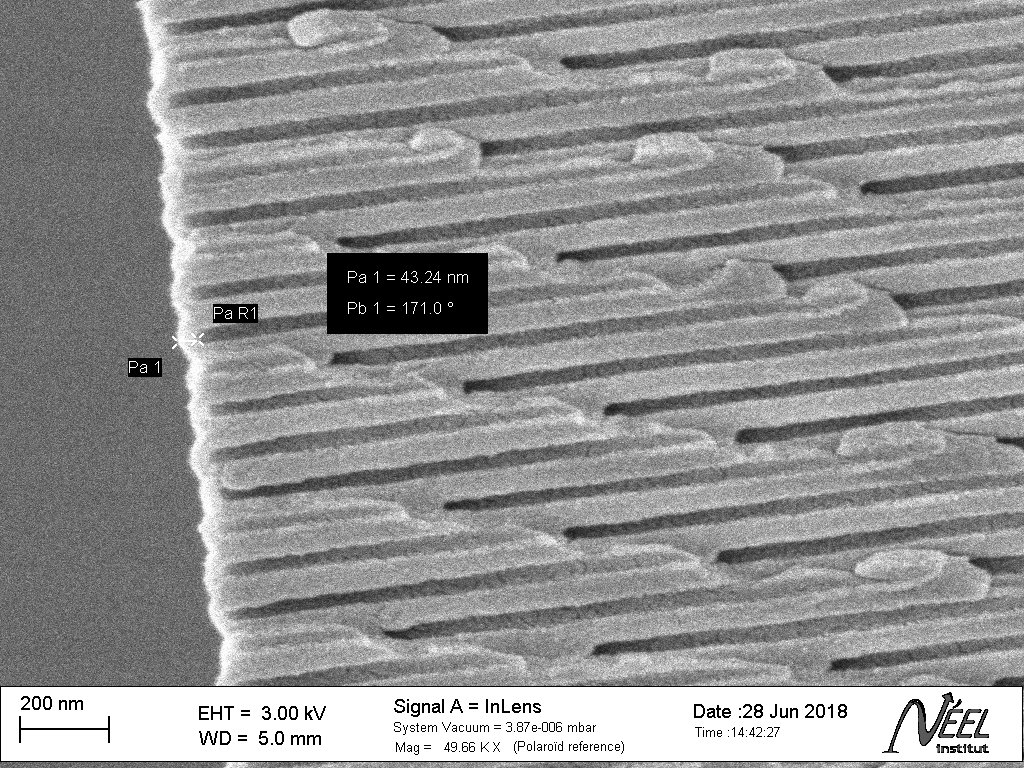
\includegraphics[width=0.45\textwidth]{images/296e_barrier_layer.jpg}
                \label{fig:296e-barrier-layer}}
                \hfill
                \subfloat[]{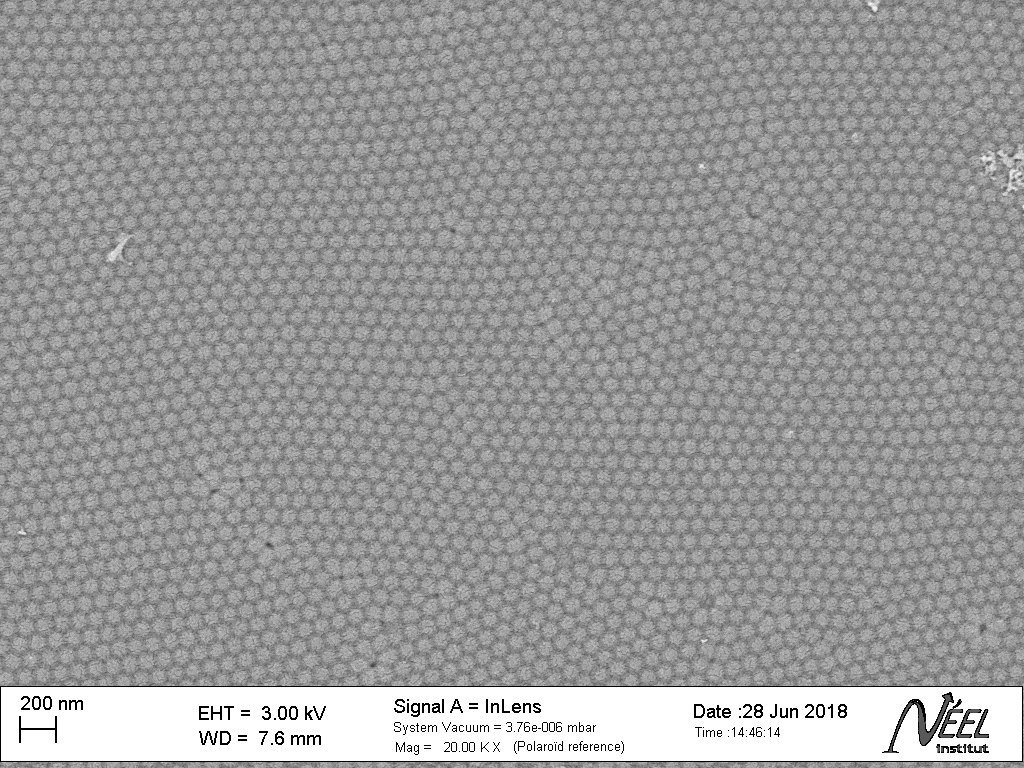
\includegraphics[width=0.45\textwidth]{images/296e_al_side.jpg}
                \label{fig:296e-al-side}}
                \caption{Electron beam microscopy images of membrane 296e' that has been floated on acid for $t_\mathrm{fl}=\SI{13}{\minute}$. \protect\subref{fig:296e-barrier-layer} shows the cross section view with the attempt to measure the thickness of the membrane's \textit{barrier layer}, while \protect\subref{fig:296e-al-side} is the aluminum side on which the membrane has been floated on.}
                \label{fig:floatin-experiment}
              \end{figure}


        \subsection{Do thinner membranes improve things?}
        \label{sec:thinner-membranes}

          Compare 295 and 296. Talk about the sharpness of both, the volumetric and the optical isotherm. Also speak about the rather broad isotherm for closed pores of 295 which is not understood. Use diameter translation by Kelvin law!!


      \section{Pore quality linked to transmission drop and hysteresis}
      \label{sec:pore-quality-link}

        As of now the shapes of the isotherms are more familiar to the reader, at this point the isotherms of the open pore membranes of wafer 295 are analysed in more detail. For this please refer to the isotherms shown in \cref{fig:295-op} of \cref{sec:wafer-inhomogeneities}. There are two isotherms that sting the eye as they do not blend in: The membranes 295c' and 295d'. Again, the analysis of membrane 295c' shall be postponed. Focusing on 295d' shows that its isotherm is not only shifted to larger pressures in comparison to the other membranes, but also is the hysteresis smaller. Moreover, the transmission drops are of a smaller magnitude for membrane 295d' than for all others. As the pressures translate to diameters
        \begin{equation}
          d_\mathrm{pore}> \SI{60}{\nano\meter},
        \end{equation}
        \textsc{Kelvin} equation is assumed to be sufficiently correct. The isotherms of the membranes 295d' and 295g', which is from here on used as a representative of the rest of the open pores membranes of wafer 295, are plotted over a diameter axis in \cref{fig:295-d-g}. Interesting at this point is, that hysteresis is actually smaller for membrane 295g' on a \textsc{Kelvin} diameter scale. Also, the evaporation branch seems sharper which could account for less funnelled pores.
        \medskip

        Very weird stuff here... HELP???

        \subfile{tikz/graphs/295_d_g/295_d_g.tex}


      \section{Testing theory using electron beam microscopy}
      \label{sec:testing-theory}


      \section{Pore size reduction using atomic layer deposition}


      \section{Isotherms proves powerful to detect and characterize defects}
      \label{sec:theory-and-defects}

      Bring up membrane 293 (constricted pore ends) and membrane 295c (closed pores).




\end{document}
